\documentclass{article}
\usepackage[top=1in, bottom=1in, left=1.5in, right=1.5in]{geometry}
\usepackage{graphicx}
\usepackage{hhline}
\usepackage{multirow}
\usepackage{url}

\begin{document}
\title{SE101---Lab 1}
\author{Rollen D'Souza, Patrick Lam, Mahesh Tripunitara}
\date{Fall 2016\\Last Updated \today}
\maketitle

\section*{Introduction}
In the first lab you are required to implement a program that takes as input a series of characters and emits a Morse Code representation of the sequence using the built-in light emitting diode (LED). The microcontroller board houses an LED capable of illuminating in red, green and blue.  Take a moment to look at Figure~\ref{fig:tivaLayout} and familiarize yourself with the board layout.

\begin{figure}[ht]
\centering
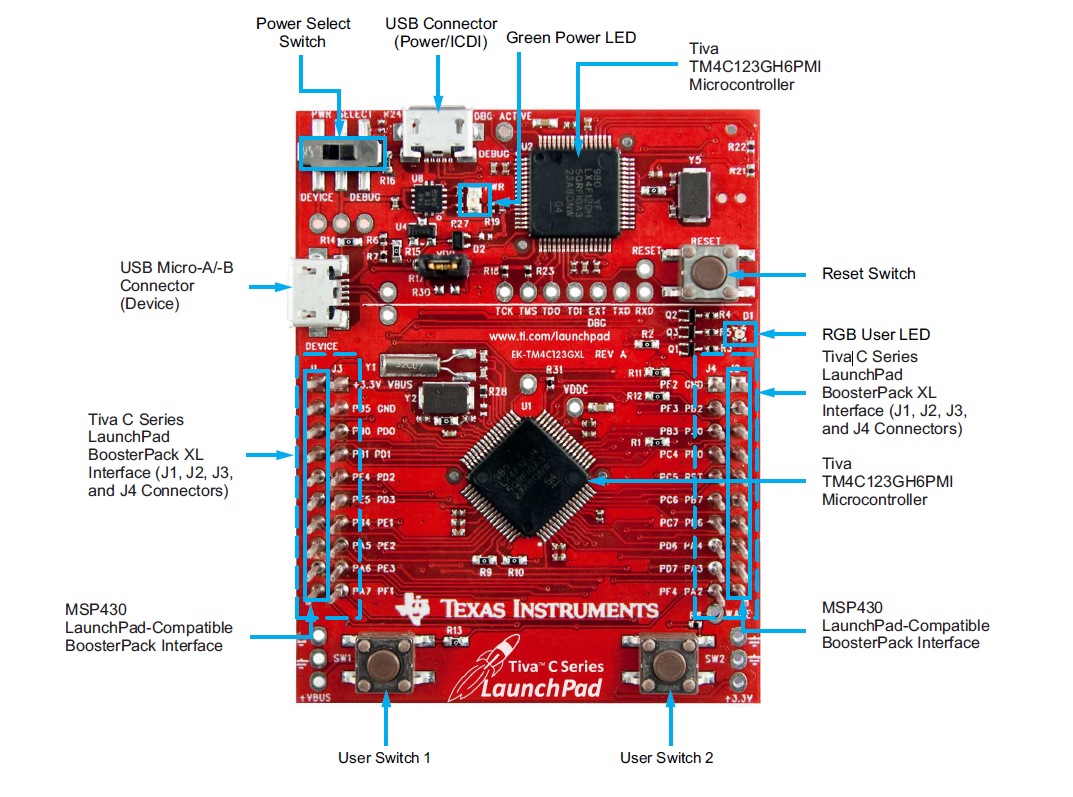
\includegraphics[width=5in]{Images/LaunchpadLayout.PNG}
\caption{Tiva C-Series TM4C123GXL Board Layout~\cite{tivaGuide}}
\label{fig:tivaLayout}
\end{figure}

\section*{Morse Code}
\emph{Morse Code} is a method of transmitting characters as a series of alternating tones---traditionally clicks (as in Figure~\ref{fig:key}), but also lights---that can be understood without the need for special equipment~\cite{wiki_morse}.  It is normally represented using a series of dots (short signal) and dashes (long signal).  Details on Morse Code, such as the specific mapping between characters and signal-sequences, can be found at the link provided in the reference.  We recommend reading the entire reference.  You will be marked against the International Morse Code chart.

\begin{figure}[ht]
\centering
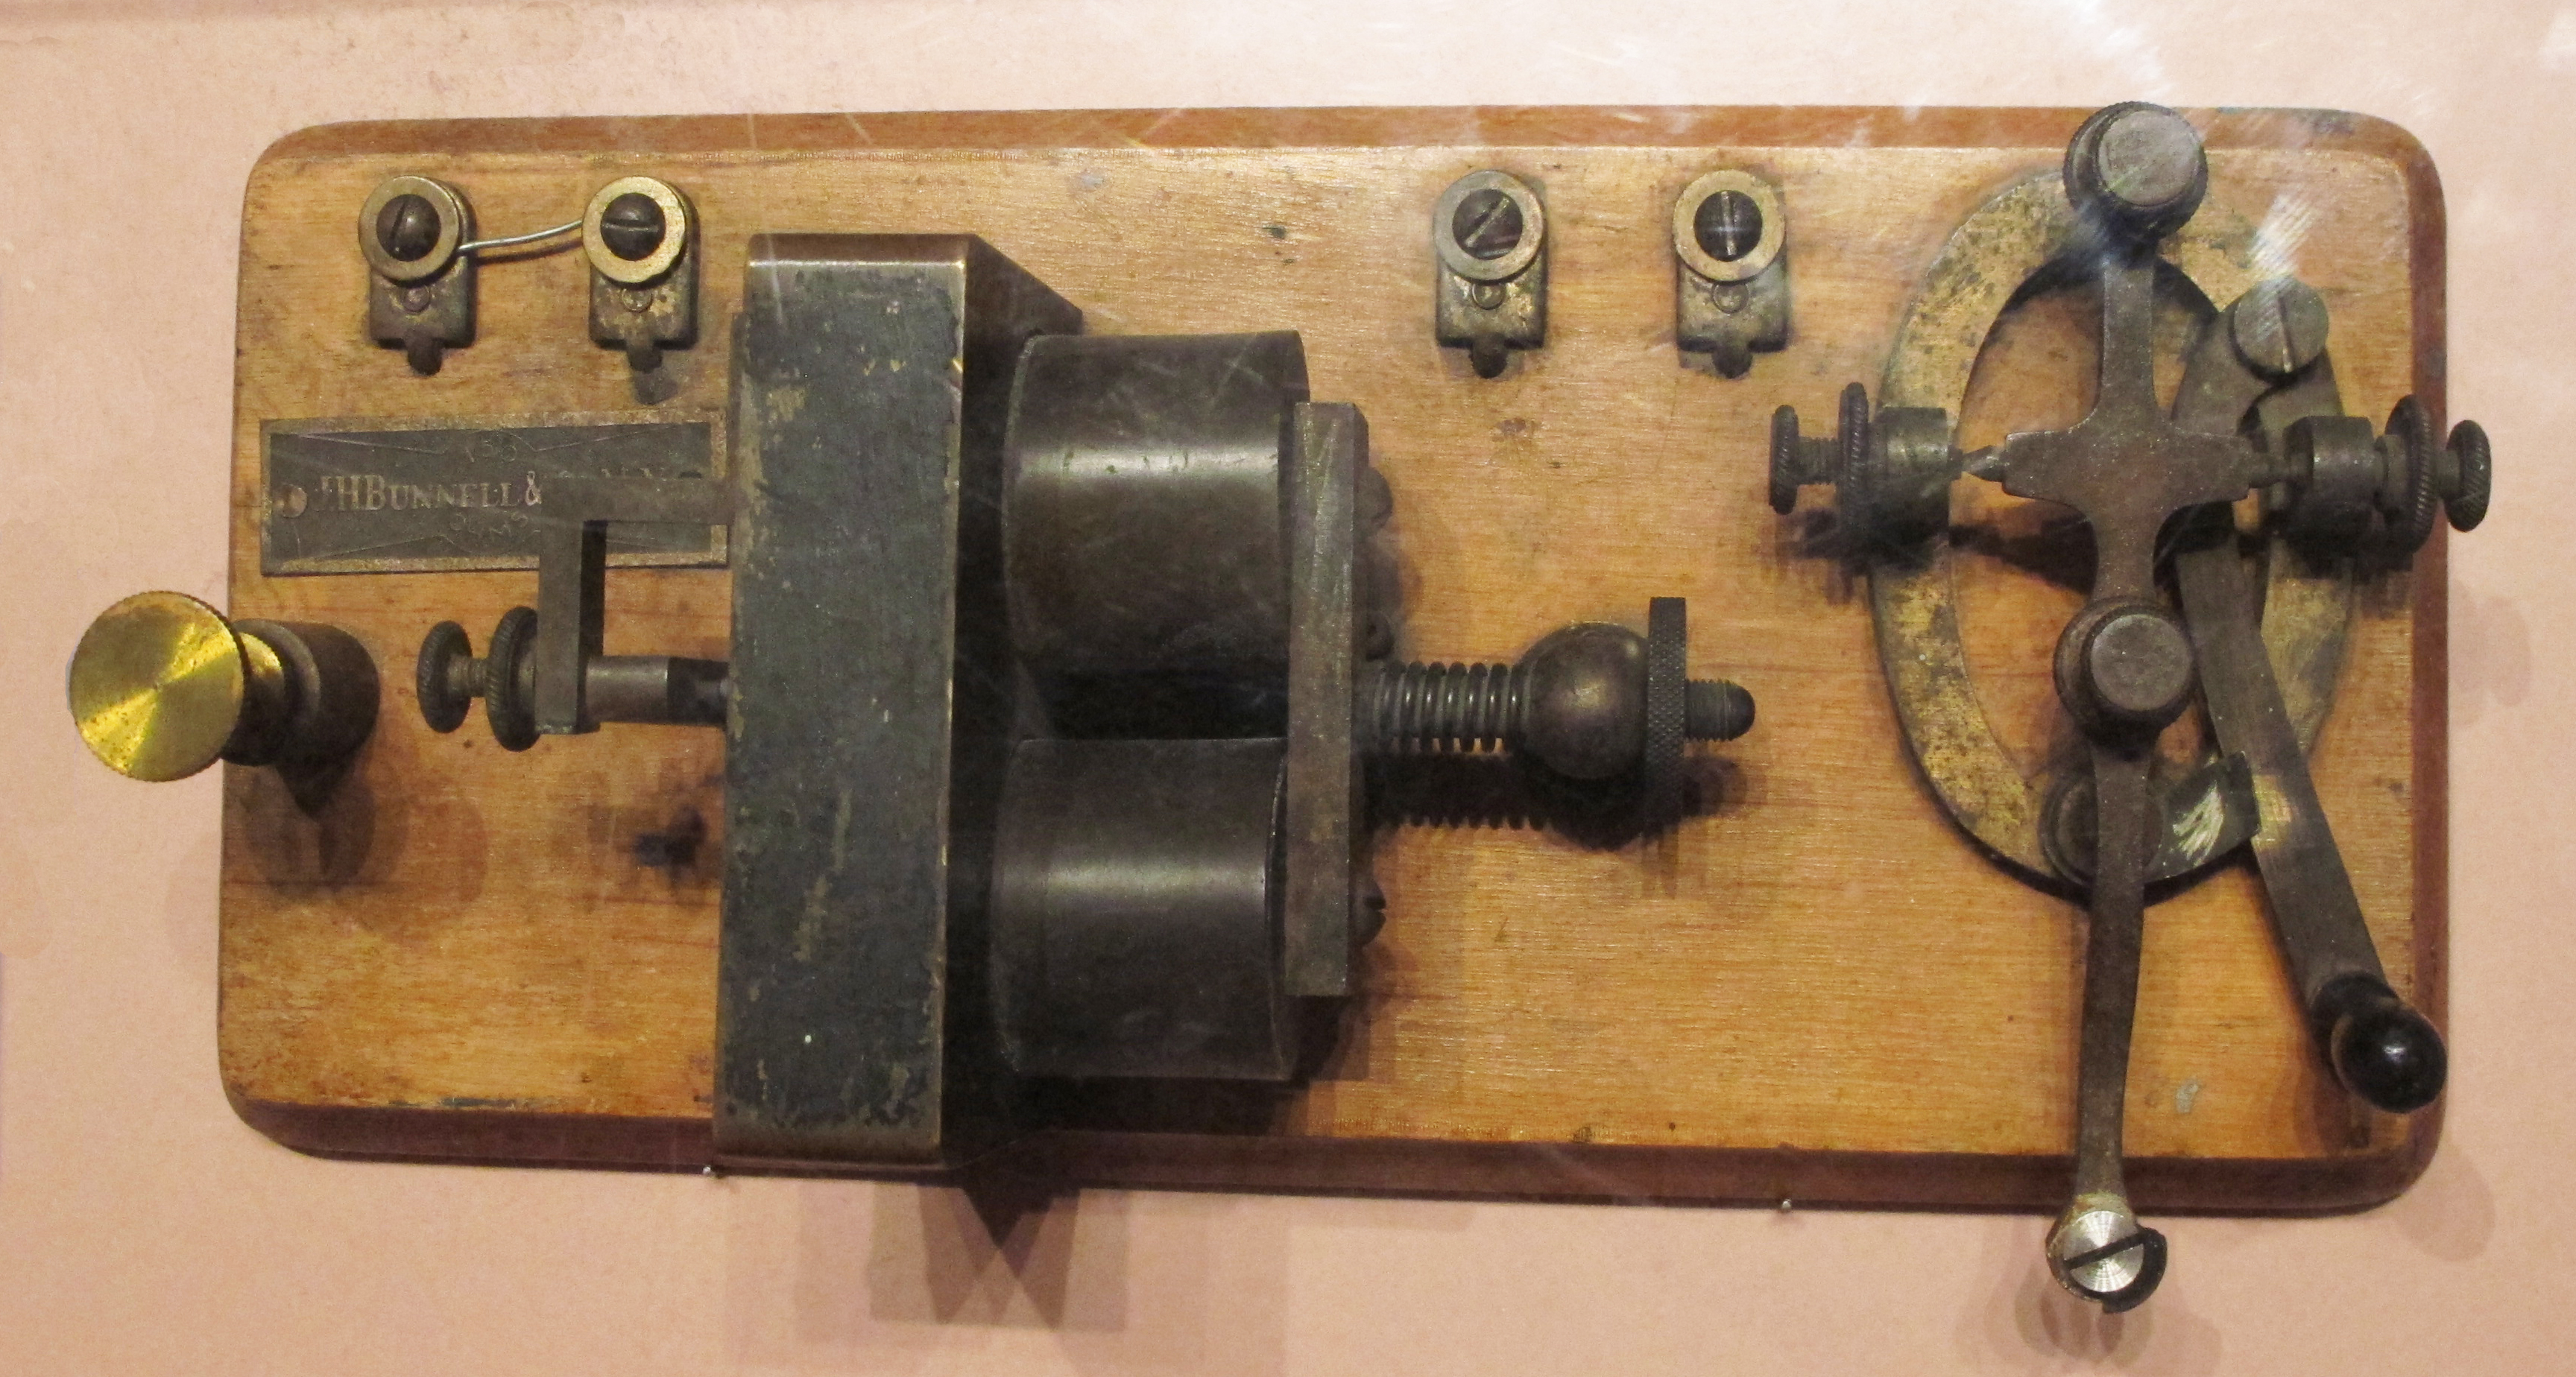
\includegraphics[width=5in]{Images/Wright_Telegraph_Key.jpg}
\caption{Wright Brothers telegraph key; By Sanjay Acharya---Own work, CC BY-SA 3.0, \texttt{https://commons.wikimedia.org/w/index.php?curid=15733842}}
\label{fig:key}
\end{figure}


\section*{Requirements}
The program must accept a line of text from the serial input and transmit the Morse encoding using the \emph{green} LED.  A line of text is delimited using the linefeed (\texttt{\textbackslash n}) character.  The program must transmit the Morse encoding of the message exactly once and then must continue to accept further messages from the user.  You must implement the morse encoding for all 26 english letters, in both upper case and lower case.  We will test atleast five characters at random as well as ill-formed input.

A dot-signal lasts one second.  A dash-signal lasts three dots.  Between signals there is a one dot length wait.  Between words there is a three dot length wait.  Punctuation and case should be ignored.


\section*{Marking Scheme}
\begin{center}
\begin{tabular}[c]{cr|c}
&\textbf{Criteria} & \textbf{Mark Contribution} \\ \hline
\multirow{3}{*}{Correctness} 
	& Correct Morse Code & 10 \\
	& Handles Ill-Formed Input & 5 \\

\multirow{4}{*}{Style} 
	& Naming & 1 \\
    	& Whitespace Usage & 1 \\
	& Easy to Modify & 1 \\
	& Use of Control Flow and Types & 1 \\
	& Use of Source Control & 1 \\ \hhline{==|=}
	
& Total & 20 \\ 
\end{tabular}
\end{center}

\section*{Submission}
You must submit your assignment using the ECE SVN (subversion) repository.  You are graded on your use of Subversion.  We expect to see at least two non-trivial commits. Trivial commits are those that consist of at most changes to whitespace.

There will be a separate document on how to use ECE SVN.

Please commit your solutions to:

\begin{center}
\url{https://ecesvn.uwaterloo.ca/courses/se101/2016/YOUR\_WATID/lab1}
\end{center}

where you replace ``YOUR\_WATID'' with your WatID (e.g. p23lam). Email Patrick Lam if you can't commit to that address.

\section*{Tips}
\begin{itemize}
	\item Use Energia's \texttt{Serial} library.
	\item Energia's Serial Monitor supports different line endings.  Be sure to select linefeed only!
	\item Consider how this lab can be broken into components.
	\item What we mean by ``easy to modify'': Can we easily remove some components of your lab for use in a different program?
	\item GCC supports encoding numbers in binary representation like so: \texttt{0b101010111}.
\end{itemize}

\begin{flushleft}
\begin{thebibliography}{1}

\bibitem{tivaGuide}
	Texas Instruments.
	(2014).
	\emph{Tiva\texttrademark C Series TM4C123G Launchpad Evaluation Board User's Guide} [PDF].
	Available: \url{http://www.ti.com/lit/pdf/spmu296}

\bibitem{wiki_morse}
	Wikipedia.
	(2016).
	\emph{Morse Code - Wikipedia} [Online].
	Available: \url{https://en.wikipedia.org/wiki/Morse_code}

\end{thebibliography}
\end{flushleft}

\end{document}
